\documentclass[11pt]{article}
\usepackage[utf8]{inputenc}
\usepackage{amsmath}
\usepackage{titlesec}
\usepackage{titling}
\usepackage{geometry}
\usepackage{graphicx}
\usepackage{hyperref}
\usepackage{fancyhdr}
\usepackage{wallpaper}
\usepackage{afterpage} 
\usepackage{pagecolor} 
\usepackage{multirow}
\usepackage{wrapfig}
\usepackage{lipsum} 
\usepackage{url}
\usepackage[toc,page]{appendix}
\usepackage{mdframed}
\usepackage{pgfgantt}
\usepackage{tabularx}
\usepackage{graphicx}

% Define colors
\usepackage{xcolor}
\definecolor{myblue}{RGB}{33, 66, 99}
\definecolor{mygray}{RGB}{169, 169, 169}
\definecolor{darkbluegrey}{RGB}{44, 62, 80} 

% Page styling
\pagestyle{fancy}
\fancyhf{}
\renewcommand{\headrulewidth}{0pt}
\renewcommand{\footrulewidth}{0pt}
\fancyfoot[C]{\thepage}
\renewcommand{\familydefault}{\sfdefault}

% Define a command for section headers
\titleformat{\section}
  {\color{myblue}\normalfont\Large\bfseries}
  {\color{myblue}\thesection}{1em}{}

% Define a command for subsection headers
\titleformat{\subsection}
  {\color{myblue}\normalfont\large\bfseries}
  {\color{myblue}\thesubsection}{1em}{}

% Adjust page margins
\geometry{a4paper, margin=1in}

% make references clickable
\hypersetup{
    colorlinks=true,
    linkcolor=blue,
    filecolor=magenta,      
    urlcolor=cyan,
}

\begin{document}

% Change the background color of the first page
\pagecolor{darkbluegrey}
\afterpage{\nopagecolor}

% Add a background image
\ThisCenterWallPaper{0.75}{./image/ferrofluide.png}

\begin{titlepage}
  \vspace*{\stretch{1}}
  \begin{center}
    \textcolor{white}{\textbf{\Huge Final Report}}\\
    \vspace{1cm}
    \textcolor{white}{\Large Spiking Neural Networks\\Sound Detection and Classification}
    \vspace{3cm}
  \end{center}
  \vspace*{\stretch{2}}
  \begin{center}
    \textcolor{white}{
      \textbf{COURREGE Téo}\\
      \textbf{GANDEEL Lo'aï}\\
      \vspace{1cm}
      \Large Date: \today}
  \end{center}
  \vspace*{\stretch{1}}
\end{titlepage}

\newpage

\tableofcontents

\pagebreak

\listoffigures

\pagebreak

\listoftables

\pagebreak

\section{Introduction}

\begin{figure}[ht]
  \begin{minipage}[b]{0.45\textwidth}
    In the last report, we explored the foundational aspects of Spiking Neural Networks (SNNs) and their potential applications, focusing on audio classification tasks. We delved into the theoretical underpinnings of SNNs, studying various neuron models and encoding methods such as rate, latency, and frequency coding. Additionally, we addressed challenges related to data preprocessing, verification, and the reconstruction of audio signals using Mel-frequency cepstral coefficients (MFCCs).
  \end{minipage}
  \hfill
  \begin{minipage}[b]{0.5\textwidth}
    \centering
    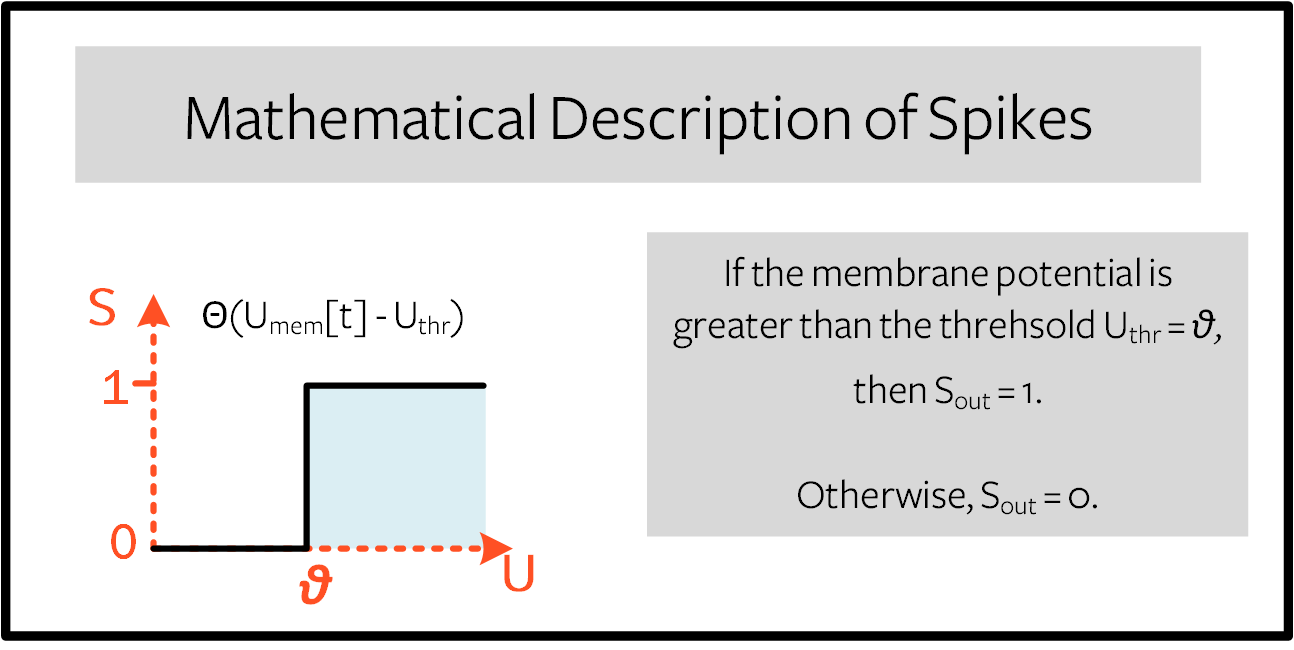
\includegraphics[width=\textwidth]{./image/spike_description.png}
    \caption{Mathematical description of a Spike}
  \end{minipage}
\end{figure}

Building upon this foundation, the current report will delve deeper into the intricacies of SNNs, specifically addressing the non-differentiability issue inherent in these networks. Non-differentiability poses a challenge in applying traditional gradient-based optimization techniques commonly used in training Artificial Neural Networks (ANNs). We will explore strategies to tackle this issue and optimize SNNs effectively.

Furthermore, we will introduce the concept of Convolutional Spiking Neural Networks (CSNNs), extending the discussion beyond simple SNN architectures. CSNNs leverage the spatial hierarchies present in convolutional neural networks (CNNs) and integrate them with the temporal dynamics of SNNs. This fusion holds promise for tasks like image recognition, where both spatial and temporal features play crucial roles.

In the practical implementation section, we will present a small program showcasing our results. This program will include the application of CSNNs in a specific task, demonstrating the capabilities and potential advantages of this hybrid architecture.

Throughout this report, our aim is to provide a comprehensive understanding of the advancements and challenges in the realm of Spiking Neural Networks, offering insights into their unique characteristics and applications.

\pagebreak 

\section{Reminder on Spiking Neural Networks}

\subsection{Spikes encoding}

The idea behind spikes is simple: we need to encode some data (let's say an image) into some other kind of data that has a temporal dependency. To do so, we will need to define time steps, a number of steps, and a threshold. 
In a rate encoding scheme, we take the values of the pixels of the image and make them pass through a function that will output or not a spike (for example, a Bernoulli function).

\begin{figure}[ht]
  \centering
  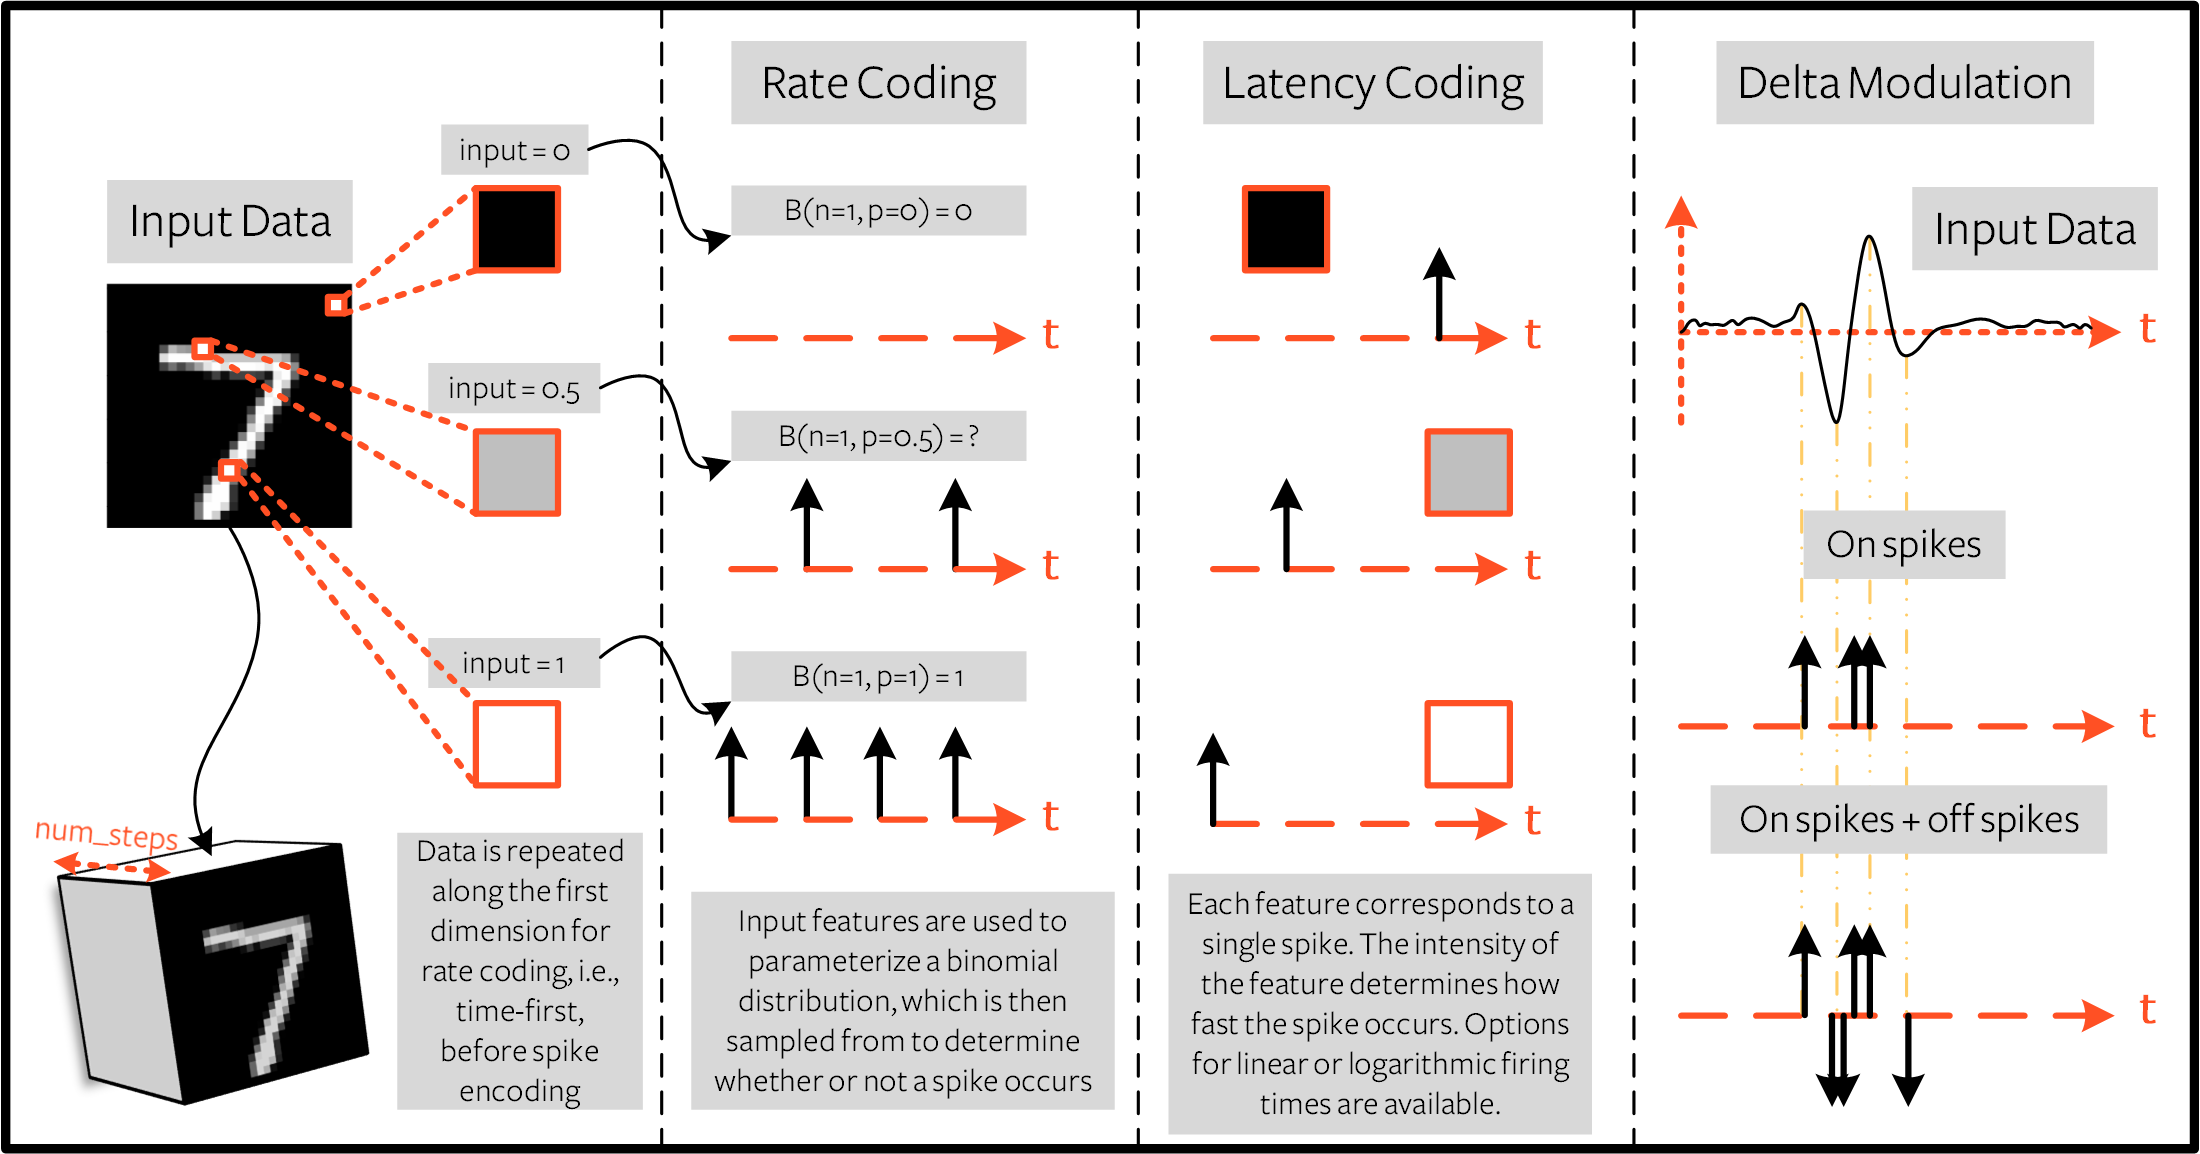
\includegraphics[width=\textwidth]{./image/spikeconv.png}
  \caption{Spike encodings of an image}
\end{figure}

Let's say we have a white pixel (value close to $1$) and a black pixel (value close to $0$). We will then pass these values through a Bernoulli function with a threshold of $0.5$. If the value is above $0.5$, we will output a spike ($1$); if not, we will output $0$.
In doing this same procedure for all the pixels of the image, for all the time steps until the number of steps, we will have a temporal dependency of the image that, when combined, can approximate the original image.

\pagebreak

\section{Non-differentiability issue}

\begin{wrapfigure}{r}{0.6\textwidth}
  \centering
  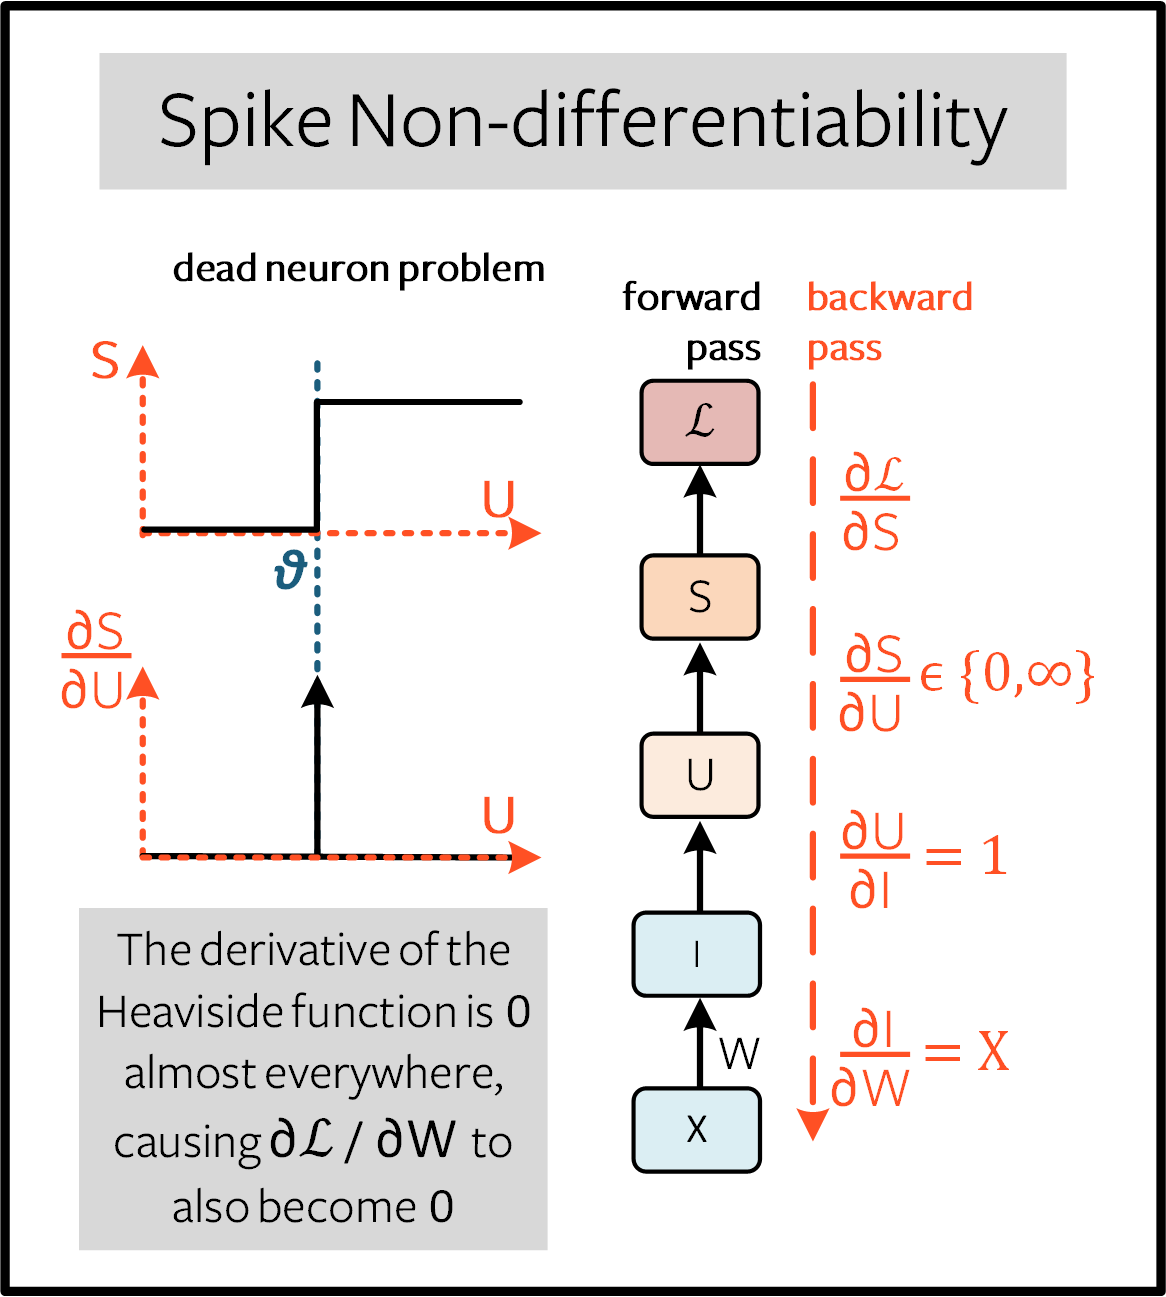
\includegraphics[width=0.6\textwidth]{./image/non-differentiability.png}
  \caption{Dead neuron problem}
\end{wrapfigure}

To train a spiking neural network, we aim to adjust the weights based on the loss gradient, minimizing the overall loss. Backpropagation achieves this through a chain of derivatives:

$$
\frac{\partial \mathcal{L}}{\partial W} =
\frac{\partial \mathcal{L}}{\partial S}
\underbrace{\frac{\partial S}{\partial U}}_{\{0, \infty\}}
\frac{\partial U}{\partial I}
\frac{\partial I}{\partial W}
$$

Here, $\mathcal{L}$ is the loss, $W$ represents weights, $S$ is the output, $U$ is the activation function, and $I$ is the input.

The challenge lies in the term $\frac{\partial S}{\partial U}$, which takes values between $0$ and $\infty$. The derivative of the Heaviside step function from the input ($U$) is the Dirac Delta function. This function is $0$ everywhere except at the threshold $\theta$, where it tends to infinity. Consequently, the gradient is often nullified to zero (or saturated if $\theta$ precisely aligns with the threshold), hindering learning. This issue is commonly known as the \textbf{dead neuron problem}. There are multiple ways to address this issue.

\subsection{Surrogate Gradient}

One way to address this non-differentiability issue would be to compute a gradient on a "relaxed" version of the non-differentiable function. This would mean approximating the Heaviside step function $S(U)$ with a differentiable function $f(U)$, such as the sigmoid function or the $\arctan$ function. For example:

\begin{figure}[ht]
  \begin{minipage}[t]{0.5\textwidth}
    \vspace{40pt} % Adjust this value as needed
    $$\begin{aligned}
        S(U) & \approx \frac{1}{1 + e^{-\beta(U - \theta)}}       \\
             & \text{Or alternatively}                            \\
        S(U) & \approx \frac{1}{\beta} \arctan(\beta(U - \theta))
      \end{aligned}$$
  \end{minipage}
  \hfill
  \begin{minipage}[t]{0.45\textwidth}
    \vspace{0pt} % Adjust this value as needed
    \centering
    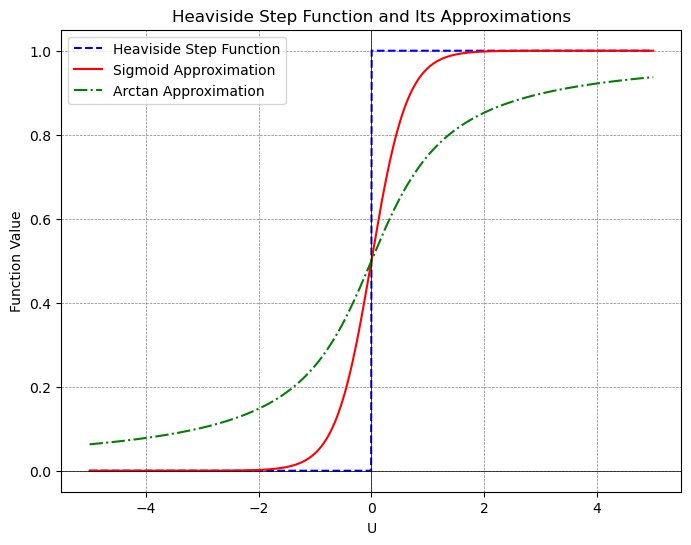
\includegraphics[width=\textwidth]{./image/approx_surrogate.png}
    \caption{Visualization of the Heaviside step function approximation}
  \end{minipage}
\end{figure}

\subsubsection{Loss function treatment}

In order for this to be taken into account in the loss function (and because we now have to take the time as a parameter), we have to perform an operation on the loss function for all its time steps.

$$ \frac{\partial \mathcal{L}}{\partial W}=\sum_t \frac{\partial\mathcal{L}[t]}{\partial W} =
\sum_t \sum_{s\leq t} \frac{\partial\mathcal{L}[t]}{\partial W[s]}\frac{\partial W[s]}{\partial W}$$

\section{Convolutional Spiking Neural Networks}

\section{Practical implementation}
\end{document}
